\documentclass{clv3}
\usepackage{booktabs,caption}
\usepackage{threeparttable}
\usepackage{hyperref}
\usepackage{xcolor}
\usepackage{multirow}
\usepackage{graphicx}
\usepackage{textcomp}
\definecolor{darkblue}{rgb}{0, 0, 0.5}
\hypersetup{colorlinks=true,citecolor=darkblue, linkcolor=darkblue, urlcolor=darkblue}

\bibliographystyle{compling}


\runningtitle{Predicting age in social media}

\runningauthor{Lorien Verachtert}
\issue{05}{19}{2017}
\begin{document}

\title{Predicting age in social media: an exploratory approach}


\author{Lorien Verachtert}
\affil{University of Antwerp}



\maketitle

\begin{abstract}
This article describes a supervised machine learning project which aimed at an automated classification of text in social media  for the purpose of author profiling. The considered profiling dimension in this project is the aspect age. The approach to the project is exploratory, because we combine ideas from previous research. The results of our experiments are similar to those of earlier study's.
\end{abstract}

\section{Introduction}
\subsection{World Wide Web and social identity}

The explosion of  online  communication  has  increased  the  need  for  more and better  analysis  of  web  content. This implies that the identification of the author of a certain text has a growing importance. Much about a person's social identity, like gender and age, can be revealed by his or hers language use \citep{nguyen2013old}. That is why automatically  predicting  an author's identity from his writings has a lot of potential. There are two main task in identifying  an author. On the one hand you have authorship attribution, where you get a closed set of candidate authors and need to identify which one of them is the author of an anonymous text.  On the other hand you have author profiling which distinguishes between classes of authors, rather than between individual authors. Author profiling can be used to determine various author aspects like gender, age, native language and personality type and can be used in various fields \citep{rangel2013overview}. For example, Internet sources such as email, blogs, forums, tweets provide an  attractive  communication  medium  for criminal activity. In forensic linguistics, determining the linguistic profile of the author of a suspicious text can help narrowing down the suspect list \citep{abbasi2005applying,estival2007author,rangel2013overview}. Another area where author profiling can provide valuable information is in marketing. It can be interesting for a business to know what types of people buy their products or dislike them \citep{glance2005deriving,rangel2013overview}.

\subsection{PAN 2013}

A shared task that worked on this problem of author profiling was a part of the PAN 2013 \footnote{http://pan.webis.de/clef13/pan13-web/}evaluation lab on uncovering plagiarism, authorship, and social software misuse. PAN is part of the Conference and Labs of the Evaluation Forum (CLEF). The author profiling task dealt with the classification of texts into classes based on the stylistic choices of their authors and considered the gender and age aspects of the author profiling problem. 

\subsection{Current project}
In this paper, a project inspired by the PAN 2013 shared task, is presented which aimed at an automated classification of text in social media  for the purpose of author profiling. The considered profiling dimension in this project is the aspect age. The dataset used here is based on the data provided by the PAN 2013 committee. Further are the conducted experiments based on various machine learning algorithms and combinations of features described by the participants of the shared task \citep{rangel2013overview}. We expect results similar to those of the PAN participants. But this project is not a replication of a previously performed machine learning experiment. Therefore, it is necessary to note that we can not make a full comparison with other results because of the new subset that is being used, the different composition of the feature set and another combination of feature selection method and classifier. What follows is an overview of previous research done in author profiling and our specific take on the problem including our hypotheses (Section 2). In Section 3, the specifics of the data set are introduced. Then,  in Section 4 the system is described and the used methods are explained. After a description of the evaluation methods in Section 5, a report follows on the experimental results in Section 6. In Section 7, we discuss the project and give an qualitative error analysis. Section 8 concludes the paper with a reflection on the project and some pointers to future research.

\section{Related research}

As mentioned in Section 1, the study of the variation of linguistic features according to the author's profile is interesting for different fields. Previous research took place in study areas such as psychology, linguistics and computational linguistics. The profiling aspect age is investigated in different studies. The majority of experiments conducted in age prediction studies are supervised machine learning experiments. Mostly the goal is to predict an age range, so the classification of texts is in age categories. In many studies there are three categories considered: 10s ([13-17]), 20s ([23-27]), 30s and more ([33-47]) \citep{argamon2009automatically}

\citet{schler2006effects} investigated age and gender prediction on the basis of a blog's vocabulary. They found that bloggers' use of prepositions and articles increased with their age, while the use of pronouns and negation decreased. This supports the use of Part of Speech (POS) n-grams as a feature for age. The use of unigrams of LIWC word classed as a feature, showed them that 10s talk a lot about friends and school, 20s about college and 30s about their job and marriage. When style and content features were used together, their model reached an overall accuracy of 76.2\%. They were able to distinguish 10s from 30s with an accuracy above 96\% and 10s from 20s  with an accuracy of 87.3\%. A notable finding is that 30s are often misclassified as 20s. \citet{argamon2009automatically} showed that a statistical analysis of word usage in text could be used to determine an author's gender, age, native language and personality type.  A part of their system performed a three-way classification on blogs based on age (10s, 20s, 30s+) and achieved an accuracy of 77.7\% when using a combination of style and content features. In line with \citet{schler2006effects}, they found that more prepositions and determiners is a characteristic of 20s and 30s. In addition, they showed that 10s are more associated with contractions (im, dont, cant). Their study showed that the strongest style-based features for the age groups 20s and 30s where identical. This features were those that distinguished both groups from the age group 10s. On a content level, the age group 10s is associated with words as haha, bored, or school. Bar, job, office are words connected to 20s, and children, wife, husband are connected to 30s. \citet{nguyen2013old} studied the correlations between language features and age in Twitter tweets. They approached age prediction in three different ways: classifying users into age categories, by their stage of life (secondary school student, college, employee) and predicting their exact age. They concluded that the higher the age, the more users tend to use more complex language which results in longer tweets, longer words and more prepositions. In line with \citet{schler2006effects} and \citet{argamon2009automatically}, \citeauthor{nguyen2013old} found that when age goes up, their system underpredicted the age. They derived from this result that most change in language occurs in the younger ages, while at the older ages most variables barely change. For the classification in age categories their model performed with a macro F-score of 0.77, for the classification in stages of life with a macro F-score of 0.68 (multi-classification). The prediction of the exact age was done with regression and reached a mean absolute error of less than 4 years. In line with the findings of \citet{schler2006effects,argamon2009automatically} and \citet{nguyen2013old} we assume the following two hypotheses.  
First, we expect that a combination of numeric features, word n-grams and POS n-grams will outperform the baseline classifier and boost the performance in our experiment. Second, we expect that the distinction between 20s and 30s will be harder, which will lead to more misclassifications in those two groups. 
 In the discussion (Section 7) we will try to feedback our results to the papers of some participants of the PAN 2013 task and to the above mentioned researchers.   

\section{Data}
As mentioned before, the training dataset used for this experiment is based on the  data provided by the PAN 2013 evaluation lab. The training dataset for PAN 2013 consists of XML files containing the conversations in HTML format (see figure \ref{Fig.1}). A conversation in this case is a post from a public repository such as Netlog. A file contains one or more conversations from one author in particular and is labeled with language (English - Spanish), gender (male-female) and age group (10s: 13-17, 20s: 23-27 and 30s: 33-47).  The filename provides also information about  the language, gender and age group, which facilitates file tasks. The documents are divided into two separate  folders  based on the language. To preserve a real-world scenario, a number of sexual predator conversations is included in the data. The data are balanced for gender, but unbalanced for age.

For this project,  only the English data for age prediction is used. The English corpus incorporates a total of 236 000 authors (XML-files) containing 413 564 conversations and 180 809 187 words. In the English data set are 164 authors with sexual predator conversations included. The detailed distribution of the English data is given in table \ref{table1}. In the present project, a subset is taken from the English age prediction data. The subset consists of 15 000 authors, 5000 randomly sampled authors of each age group. There is no division in training and test set, because of the use of tenfold cross validation. A simple distribution of the subset is given in table \ref{table2}.  Gender is not taken into account. The focus is on age prediction, regardless of gender.

\begin{table}[h]
\centering
\caption{Statistics of experimental data for English (Patra et al., 2013)}
\label{table1}
\begin{threeparttable}
\begin{tabular}{|l|l|l|}
\hline
Age group & Gender                                                & Number of authors                                                 \\ \hline
10s       & \begin{tabular}[c]{@{}l@{}}Male\\ Female\end{tabular} & \begin{tabular}[c]{@{}l@{}}8 600\\ 8 600\end{tabular}             \\ \hline
20s       & \begin{tabular}[c]{@{}l@{}}Male\\ Female\end{tabular} & \begin{tabular}[c]{@{}l@{}}42 900 (72)\\ 42 900\end{tabular} \\ \hline
30s       & \begin{tabular}[c]{@{}l@{}}Male\\ Female\end{tabular} & \begin{tabular}[c]{@{}l@{}}66 800 (92)\\ 66 800\end{tabular}      \\ \hline
\end{tabular}
\begin{tablenotes}
	\item[a] Note: numbers inside parentheses for male 20s and 30s correspond to the number of authors of sexual predator conversations
 \end{tablenotes}
     \end{threeparttable}
\end{table}

\begin{table}[]
\centering
\caption{Statistics of subset of experimental data for English}
\label{table2}
\begin{tabular}{|l|l|l|}
\hline
Age group & Number of conversations & Number of authors \\ \hline
10s       & 8002                    & 5000              \\ \hline
20s       & 8849                    & 5000              \\ \hline
30s       & 8464                    & 5000              \\ \hline
All       & 25 315                  & 15 000            \\ \hline
\end{tabular}
\end{table}

\section{System description}
\subsection{Preprocessing}
The first step in the data preprocessing phase was the making of a data subset. This step is in line with the study of \citet{patra2013automatic}. They also used a subset of the English corpus. The subset was made in order to reduce dimensionality. As you can  see above in tables \ref{table1} and \ref{table2}, the data went from 236 000 files to 15 000 files.  The XML-files contained a lot of information, but for this project, only the information about age and the conversations itself were valuable. That is why age and text were extracted from the files and contained in a list. The next step was to clean the text. The HTML mark-up was removed using the Python library Beautiful Soup\footnote{https://www.crummy.com/software/BeautifulSoup/Download}.  Regular expressions were used to remove URLs and other unwanted characters. These two steps were in line with \citet{meina2013ensemble} and \citet{patra2013automatic}. We also noticed that many conversations seemed to be spam. Like \citeauthor{meina2013ensemble} suggested, this could be due to chatterbots producing  text for commercial purposes. Due to time restrictions spam-like conversations weren't filtered out. \citet{rangel2013overview} reported that there are some conversations of sexual predators introduced into the PAN data. Because of the small number of sexual predators conversations compared to the total amount of conversations, we did not take into account the possibility of  the presence of such conversations in our subset. The effect of spam and texts of sexual predators on the data will be discussed in Section 7. The final step was to dump the cleaned data into a json-file.

\subsection{Feature engineering}
Some of the feature extraction procedures required word and sentence tokenization and part-of-speech tagging. These tasks weren't performed during the preprocessing phase and thus implemented in the feature extraction using the NLTK tools from the NLTK Python library \citep{bird2009natural}.

We considered three different types of features. The used features are shown in table \ref{table3}. First we have a few numeric \footnote{we chose this name because its features are based on simple number calculations} features: type token ratio, total number of words, average word length and average sentence length. Type token ratio (TTR) is a good feature to find something out about the vocabulary richness of a conversation. A high TTR indicates a large amount of lexical variation and a low TTR indicates relatively little lexical variation. We chose to use the average sentence length because \citet{rustagi2009stylometric} reported it as a good indicator of age, as there is an increase of the average sentence length with age. When the average sentence length is higher, the total amount of words in a conversation will also be higher. That is why we use the total number of words in a conversation as a feature. We also added average length of a word because \citet{kocherdistance} report that younger people tend to use less complex words, which can be evaluated by the mean number of letters per word. All the numerical features have as result a float or an integer and are per feature turned into a vector of features for each conversation. The second one, on the word-level, is the relative frequency of word n-grams. Therefore we use word unigrams, to test the isolated words and bigrams to catch some context around the words. We also experimented with word trigrams but this led to poorer results, so they were omitted.  For each conversation, the number of occurrences of each word uni-, and bigram is counted and the obtained frequencies are then turned into a vector of features. The third type of feature, on the syntax level, is the relative frequency of part-of-speech n-grams. \citet{baayen1996outside,stamatatos2001computer} and \citet{koppel2002automatically} showed that the use of POS n-grams is a simple but relatively efficient way to capture syntactic information for the use of distinguishing writing styles. The use of the relative frequency of n-grams is also in line with the study of \citet{meina2013ensemble} and \citet{santosh2013author}. An n-gram is in this case a contiguous sequence of n POS tagged words from a given sequence. We count the number of occurrences of each POS uni-, and bigram in each conversation. The obtained frequencies are then again employed to generate a vector of features for each conversation. 

\begin{table}[h]
\centering
\caption{Feature set}
\label{table3}
\begin{tabular}{|l|l|l|}
\hline
Numerical (word-based) features & Relative frequency of n-grams & Relative frequency of POS n-grams \\ \hline
TTR (type token ratio)          & Unigrams                      & Unigrams                          \\ \hline
Total number of words         & Bigrams                       & Bigrams                           \\ \hline
Average sentence length         &                               &                                   \\ \hline
Average word length             &                               &                                   \\ \hline
\end{tabular}
\end{table}

\subsection{Feature selection}
The feature extraction gave us a lot of features. We wanted the strongly discriminative ones. In line with the study of \citet{cruz2013italica} the chi-square correlation measure between the features and the output classes was used to carry out the selection of features. According to a study  from \citet{zheng2004feature}, the chi-square is one of the most effective feature selection metrics for text categorization, next to information gain, correlation coefficient and odds ratios.  In statistics, the Pearson's chi-square distribution tests whether the occurrence of a feature and the occurrence of a class are independent (the Zero hypothesis). The aim is to select those features of which the occurrence is highly dependent on the class occurrence. The Chi- square for feature selection is a two-sided metric which considers the features most indicative of either positive features (membership) or negative features (non-membership).This means that two-sided metrics combine the positive and negative features, they are non-negative with the signs of features ignored \cite{zheng2004feature}. The formula for the chi-square measure is as follows:
\begin{figure}[h]
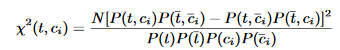
\includegraphics[width=4in]{formulechi2}
\end{figure}

Where N is the total number of documents , term t and category c.
We used the Chi2 function from Scikit learn with the SelectKbest class.  This class allows us to get the k best features. We experimented with a window of 1000, 3000, 5000 and, finally the one with the best results, the 10 000 best features.

\subsection{Learning method}
This paper deals with a multi-class classification problem. We have three classes, the three age groups: 10s, 20s, 30s. Each conversation can only be assigned to one class, it's most probable label. As described in the feature extraction, we represent a document (conversation) as a numerical vector X = (x1,..,xi,...,xn), where n is the number of features and xi is the relative frequency of feature i in the document.

The prediction of the author's age is done by training a classifier. \citet{argamon2009automatically} say that the most effective multi-class classifiers for author profiling all have the same structure. First they learn a weight vector Wj = (w1j,...wij,...,wnj) for each category cj and then they assign a document, X, to the class for which the inner product Wj*X is maximal. We experimented with three different classifiers, capable of performing multi-class classification: Decision Tree, Random Forest and Linear Support Vector Classifier (SVC). The final experiments were conducted with the best performing classifier, which was the LinearSVC method with standard parameters from the Scikit-learn library \cite{pedregosa2011scikit}. The LinearSVC is a Liblinear\footnote{https://www.csie.ntu.edu.tw/~cjlin/liblinear/} based Support Vector Machine Classifier and as such attempts to divide the data space with the use of linear delineations between the different classes. The key in a SVM classifier is to determine the optimal boundaries between the different classes. The output of the linear predictions is defined to be p=A.X+b, where X=(x1...xn) is the normalized document word frequency vector, A=(a1...an) is a vector of linear coefficients with the same dimensionality as the feature space, and b is a scalar. A natural interpretation of the predictor p = A.X+b in case of categorical class labels would be as a separating hyperplane between the different classes. It uses a One-vs-the rest multi-class reduction to determine the multi-class strategy, in contrast to SVC which uses a One-vs-One multi class reduction. Another difference is that LinearSVC minimizes the squared hinge loss, while SVC minimizes the regular hinge loss \citep{aggarwal2012survey,pedregosa2011scikit}.

\section{Evaluation}
The training and evaluation of the classifier is done by performing ten-fold cross-validation. We compared our model to a weighted random baseline (WRB, the sum of the squared class proportions) and a majority baseline (MAJ). The WRB is 0.33 and the MAJ is 0.35. In the evaluation we report precision, recall and F-score per class and the macro F-score for the overall performance.
\subsection*{Evaluation metrics}
The quality of the overall performance of our classification method is assessed by using macro-averaging (a measure is the average of the same measures calculated for all classes). We chose to use the macro F-score because in macro-averaging all the classes are treated equally, so it gives a sense of effectiveness on small classes. While in micro-averaging bigger classes are favored, which means that micro-averaged results are a measure of effectiveness on the large classes in a dataset \citep{sokolova2009systematic}\footnote{For formulas of the measures see Figure\ref{Fig.1} in the additional material}.The macro F-score is the harmonic mean of the macro precision and macro recall. We also report the precision, recall and F-score per predicted class.

Also confusion matrices are computed to evaluate the output of the classifier. The rows in the confusion matrix correspond to the true class of the data, i.e. the known labels. The columns correspond to the predictions made by the model, i.e. the predicted labels. The diagonal elements stand for the number (or percentage in case of normalization) of correct classifications made for each class, i.e. when the predicted label is equal to the true label. Figure \ref{Fig.3} is a confusion matrix without normalization. Because of the unbalanced distribution of the classes, a normalized confusion matrix is computed (Figure \ref{Fig.4}). The normalization is performed by class support size. This way we get a more visual interpretation of which class is being misclassified \citep{pedregosa2011scikit}. 

\section{Results}
We experimented with different combinations of features. After a final feature selection we concluded that the best feature set for our age prediction task was a set of 10 000 features, consisting of all numeric features, relative frequency of word uni-, and bigrams and relative frequency of POS uni-, and bigrams. As reported in Section 4, we tested three different classifiers on this set of which the best performing one was the LinearSVC with a macro F-score of 0.63. Table \ref{table4} reports the precision, recall, F-score per label and the macro F-score for the overall performance. In table \ref{table5} you can compare the results for the same measures but for all three classifiers and with the different SelectKbest windows.

The normalized confusion matrix indicates that 57\% of the 10s are correctly classified, 34\% labeled as 20s and a very small amount was labeled as 30s. Remarkable is that 90\% of the 20s is correctly classified and only 7\% was  labeled as 30s. The 30s seem the be the most misclassified class with only 43\% correctly classified, 53\% labeled as 20s and again was just a small amount labeled as 10s.

\begin{table}[h]
\centering
\caption{Results for LinearSVC with k = 10 000}
\label{table4}
\begin{tabular}{|l|l|l|l|l|}
\hline
Age group & Precision & Recall & F-score & Macro F-score \\ \hline
10s       & 0.88      & 0.57   & 0.69    &               \\ \hline
20s       & 0.52      & 0.90   & 0.66    &               \\ \hline
30s       & 0.74      & 0.43   & 0.54    &               \\ \hline
All       &           &        &         & 0.63          \\ \hline
\end{tabular}
\end{table}

\section{Discussion}
A direct comparison with related research is impossible because we use a different dataset (subset), other preprocessing steps, a different feature set, other learning methods and other evaluation metrics. However, if we look at the separate aspects of our system, we can conclude that our age prediction results are comparable to the results achieved by researchers mentioned in Section 2 and by the PAN participants. Our best performing classifier, a linear support vector classifier, is often mentioned in text classification studies as good performing. \citet{meina2013ensemble}, who only tested the Spanish data, also concluded that the linear SVM classifier was the best performing one, with an accuracy of approximately 0.60. \citet{cruz2013italica} reached an accuracy of 0.62 with the Liblinear SVM method. \citet{nguyen2013old} made use of the Liblinear and Scikit-learn libraries, which corresponds to our LinearSVC, and reached a macro F-score of 0.77 for the categorization in age groups and a macro F-score of 0.68 for the categorization in stages of life. We trained our classifier on a relatively simple feature set, which largely corresponds to that of \citet{santosh2013author}. They also used the frequency of word an POS n-grams, but added topic based features (LDA). We added only some easy numerical features to the n-grams,  but as we expected, our system was still able to outperform the baseline classifier and get good results. Most of the studies in age prediction report the use of a more extensive feature set with a combination of more different features. Other features that are often included for age prediction are dictionary-based, topic-specific or based on readability measures. With regard to the classification in age categories, we found that 10s are easily distinguished from 30s and relatively easy from 20s. This is in line with many previous study's, like those from \citet{schler2006effects,argamon2009automatically} and \citet{nguyen2013old}. Our confusion matrix also showed in line with the aforementioned that 30s are very often misclassified as 20s.

\subsection*{Error analysis}
As reported in the results, the correct age group was not predicted for all conversations. This can be due to various factors which will be discussed here. We will also look into other factors that might have given us a distorted picture of the results.

\subsubsection*{Effect of other variables on age  	} 
An author's identity is not solely based on his or hers age. This project isolated the aspect age, but an identity is based on the different variables that people use in order to express themselves. Other variables that may play a role are gender and social status. An author can emphasize certain identity aspects depending on what he or she wants to express in a particular situation towards a particular person \citep{nguyen2013old}. This variability can make age prediction more complicated. By focusing on age, we did not take into account the possible interactions between variables (e.g. gender and age), which may have led to misclassifications.
\subsubsection*{Spam and sexual predators}
As mentioned in the description of the data, there were conversations produced by chatterbots in our subset. This type of spam can cause unnecessary noise when training the classifier. We did not discriminate spam-like from human-like conversations during the preprocessing. Suppose that the spam had a marketing goal, then the advertisement of certain products is more oriented towards one age group than towards the other one, which means that our system may not have performed as well as it could because of the noisy spam conversations in our data. With regard to conversations of sexual predators, we already reported (Section 4) that we did not take into account the presence of such data. But if such conversations are part of our subset, they will make it harder to predict the age group correctly. The aim of sexual predators is to hide their real identity and to pretend to be someone they are not. For example, they want to present themselves as a younger person. Therefore they will change their writing style to what they think is the style of a younger writer. In fact, their writings will reflect some aspects of their own identity, but also of their fictive identity. So, this conversations can be noisy, which can lead to misclassified conversations.
\subsubsection*{High recall for 20s}
As reported in table \ref{table4}, the class 20s had a low precision of 0.52 and a very high recall of 0.90.  The opposite was true for 10s and 30s, they both had a high precision and a low recall. The classifier seems to  favor 20s, so it is probably biased towards the majority class 20s. This means that the classifier selects most of the 20s conversations (high recall), but it is not exact in the classification (low precision). The classes 10s and 30s are not often selected, but when they are selected, the prediction is rather exact. The fact that the classifier is biased, can be due to the unbalanced data set. We can say that our evaluation metrics per class produced misleading conclusions, since they did not take misclassification costs in account and were non-sensitive to class skews.
\section{Conclusion}
We performed a supervised machine learning experiment which aimed at predicting age on a subset of the English author profiling PAN 2013 shared task. Age prediction in social media is an author profiling task with a lot of potential in various fields, therefore many sectors such as marketing and forensics can benefit from research in this area.  Our results confirm prior findings that  classification of social media texts in age groups can be successful. 

Our hypothesis with regard to our feature set was correct. A combination of simple numeric features, word n-grams and POS n-grams is able to outperform the baseline classifier and boost the performance. Our system performs already quite well with a macro F-score of 0.63, but there is still a lot of room for improvement. Due to the large amount of feature vectors (10 000), our run time was rather high. So this is an example of an aspect to improve. We could try different feature selection methods in further research. With regard to the feature set, we could augment the performance by looking at deeper syntactic features and maybe even induce sentiment analysis to discover more differences in the language of different age groups. We also assumed that the distinction between 20s and 30s would be more difficult than the distinction between 10s and 20s and 30s. Therefore, we expected more misclassifications in 20s and 30s. Our results showed that 30s were indeed often misclassified, but 20s were, against our expectations, the best classified group. We supposed that this was due to the classifier being biased towards the 20s. The finding that 30s are often misclassified as 20s, but 20s are not often  labeled as 30s and the finding that a certain amount of 10s is still misclassified as 20s, will then probably also be due to this bias. In further research, we could use a bias correction function with the aim of highlighting those classification results that present moderately higher prediction rates on the minority class.  It would also be interesting to do experiments with our feature set in combination with linear regression to try predict the exact age, instead of a classification in age groups.

\starttwocolumn
\bibliography{compling_style}


\pagebreak
\clearpage

\section{Additional material}
\columnbreak
\begin{table}[h]
\centering
\caption{Overview of the results for all classifiers}
\label{table5}
\begin{tabular}{ lllllll p{10cm} }
\hline
K = N  & Classifier    & Age group                                                     & Precision                                                  & Recall                                                     & F-score                                                    & Macro F-score                                             \\ \hline
1000   & Decision Tree & \begin{tabular}[c]{@{}l@{}}10s\\ 20s\\ 30s\\ All\end{tabular} & \begin{tabular}[c]{@{}l@{}}0.49\\ 0.44\\ 0.36\end{tabular} & \begin{tabular}[c]{@{}l@{}}0.22\\ 0.28\\ 0.68\end{tabular} & \begin{tabular}[c]{@{}l@{}}0.31\\ 0.34\\ 0.47\end{tabular} & \begin{tabular}[c]{@{}l@{}}/\\ /\\ /\\ 0.37\end{tabular}  \\ \hline
5000   & Decision Tree & \begin{tabular}[c]{@{}l@{}}10s\\ 20s\\ 30s\\ All\end{tabular} & \begin{tabular}[c]{@{}l@{}}0.52\\ 0.43\\ 0.49\end{tabular} & \begin{tabular}[c]{@{}l@{}}0.37\\ 0.68\\ 0.32\end{tabular} & \begin{tabular}[c]{@{}l@{}}0.44\\ 0.53\\ 0.39\end{tabular} & \begin{tabular}[c]{@{}l@{}}/\\ /\\ /\\ 0.45\end{tabular}  \\ \hline
10 000 & Decision Tree & \begin{tabular}[c]{@{}l@{}}10s\\ 20s\\ 30s\\ All\end{tabular} & \begin{tabular}[c]{@{}l@{}}0.55\\ 0.44\\ 0.47\end{tabular} & \begin{tabular}[c]{@{}l@{}}0.39\\ 0.65\\ 0.36\end{tabular} & \begin{tabular}[c]{@{}l@{}}0.45\\ 0.52\\ 0.41\end{tabular} & \begin{tabular}[c]{@{}l@{}}/\\ /\\ /\\ 0.46\end{tabular}  \\ \hline
1000   & Random Forest & \begin{tabular}[c]{@{}l@{}}10s\\ 20s\\ 30s\\ All\end{tabular} & \begin{tabular}[c]{@{}l@{}}0.52\\ 0.44\\ 0.36\end{tabular} & \begin{tabular}[c]{@{}l@{}}0.22\\ 0.28\\ 0.70\end{tabular} & \begin{tabular}[c]{@{}l@{}}0.31\\ 0.34\\ 0.48\end{tabular} & \begin{tabular}[c]{@{}l@{}}/\\ /\\ /\\ 0.38\end{tabular}  \\ \hline
5000   & Random Forest & \begin{tabular}[c]{@{}l@{}}10s\\ 20s\\ 30s\\ All\end{tabular} & \begin{tabular}[c]{@{}l@{}}0.58\\ 0.44\\ 0.51\end{tabular} & \begin{tabular}[c]{@{}l@{}}0.40\\ 0.71\\ 0.34\end{tabular} & \begin{tabular}[c]{@{}l@{}}0.47\\ 0.54\\ 0.41\end{tabular} & \begin{tabular}[c]{@{}l@{}}/\\ /\\ /\\  0.48\end{tabular} \\ \hline
10 000 & Random Forest & \begin{tabular}[c]{@{}l@{}}10s\\ 20s\\ 30s\\ All\end{tabular} & \begin{tabular}[c]{@{}l@{}}0.63\\ 0.45\\ 0.51\end{tabular} & \begin{tabular}[c]{@{}l@{}}0.40\\ 0.71\\ 0.39\end{tabular} & \begin{tabular}[c]{@{}l@{}}0.49\\ 0.55\\ 0.44\end{tabular} & \begin{tabular}[c]{@{}l@{}}/\\ /\\ /\\ 0.49\end{tabular}  \\ \hline
1000   & Linear SVC    & \begin{tabular}[c]{@{}l@{}}10s\\ 20s\\ 30s\\ All\end{tabular} & \begin{tabular}[c]{@{}l@{}}0.81\\ 0.49\\ 0.37\end{tabular} & \begin{tabular}[c]{@{}l@{}}0.14\\ 0.27\\ 0.83\end{tabular} & \begin{tabular}[c]{@{}l@{}}0.25\\ 0.35\\ 0.51\end{tabular} & \begin{tabular}[c]{@{}l@{}}/\\ /\\ /\\ 0.37\end{tabular}  \\ \hline
5000   & Linear SVC    & \begin{tabular}[c]{@{}l@{}}10s\\ 20s\\ 30s\\ All\end{tabular} & \begin{tabular}[c]{@{}l@{}}0.85\\ 0.46\\ 0.77\end{tabular} & \begin{tabular}[c]{@{}l@{}}0.45\\ 0.91\\ 0.33\end{tabular} & \begin{tabular}[c]{@{}l@{}}0.59\\ 0.62\\ 0.46\end{tabular} & \begin{tabular}[c]{@{}l@{}}/\\ /\\ /\\ 0.55\end{tabular}  \\ \hline
10 000 & Linear SVC    & \begin{tabular}[c]{@{}l@{}}10s\\ 20s\\ 30s\\ All\end{tabular} & \begin{tabular}[c]{@{}l@{}}0.88\\ 0.52\\ 0.74\end{tabular} & \begin{tabular}[c]{@{}l@{}}0.57\\ 0.90\\ 0.43\end{tabular} & \begin{tabular}[c]{@{}l@{}}0.69\\ 0.66\\ 0.54\end{tabular} & \begin{tabular}[c]{@{}l@{}}/\\ /\\ /\\ 0.63\end{tabular}  \\ \hline
\end{tabular}
\end{table}


\clearpage
\begin{figure}[h]
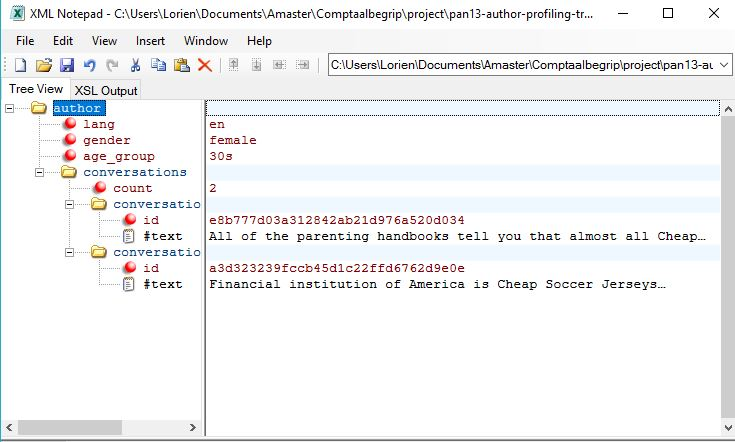
\includegraphics[width=12cm]{structuurdata.JPG}
\caption{ Example of a XML data file }
\label{Fig.1}
\end{figure}
\columnbreak

\begin{figure}[h]
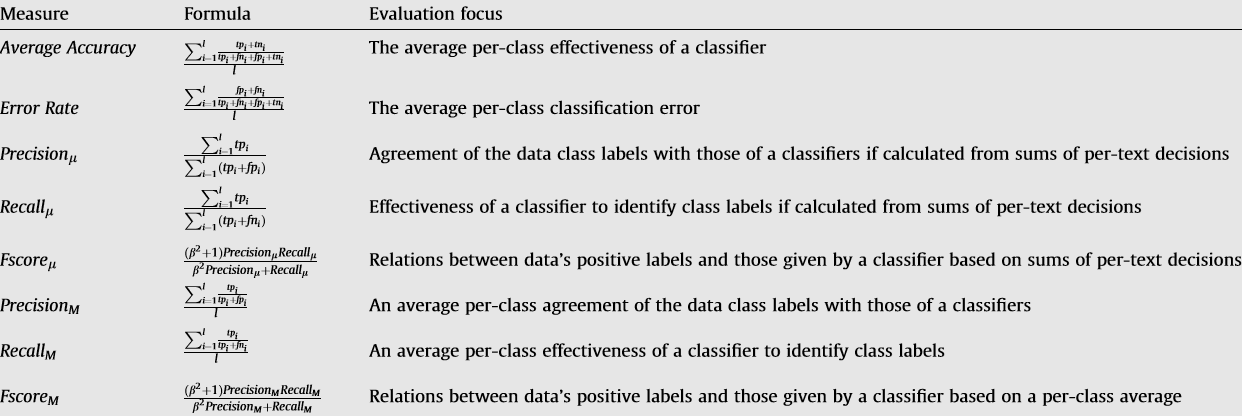
\includegraphics[width=15cm]{performancemeasures.PNG}
\columnbreak
\caption{ Measures for multi-class classification. For many classes Ci: tpi are true positive for Ci, and fpi are false positive, fni are false negative, and tni are true negative counts respectively. \textmu \space and M indices represent micro- and macro-averaging. \cite{sokolova2009systematic} }
\label{Fig.2}
\end{figure}

\clearpage
\begin{figure}[h]
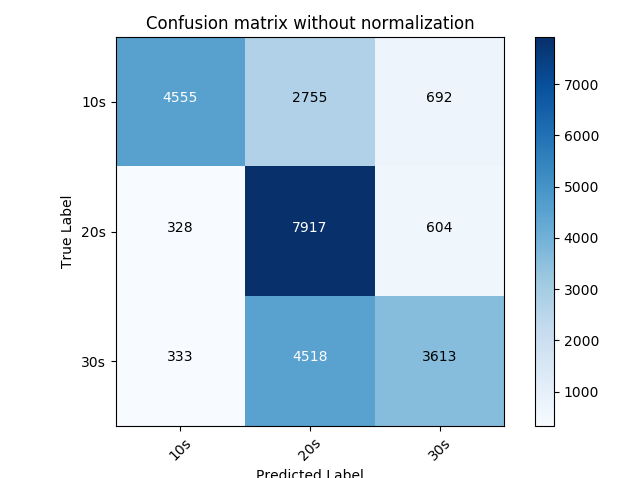
\includegraphics[width=4in]{c0.png}
\caption{ Confusion matrix of the results without normalization }
\label{Fig.3}
\end{figure}


\begin{figure}[h]
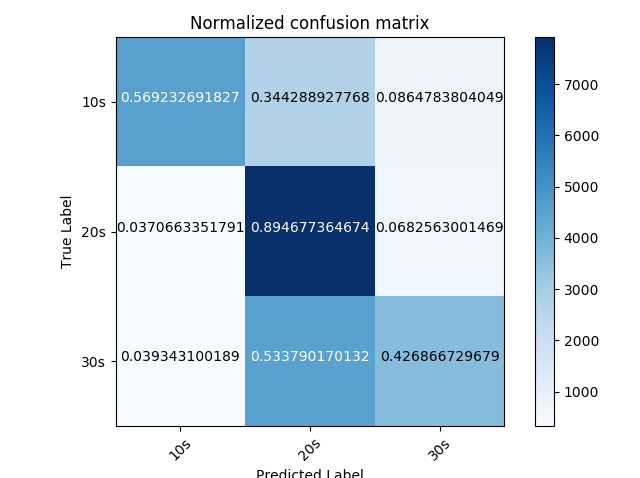
\includegraphics[width=4in]{c1.png}
\caption{ Confusion matrix of the results with normalization }
\label{Fig.4}
\end{figure}
\end{document}






